\chapter[Contraintes mésoscopiques du milieu granulaire]{Détermination du tenseur des contraintes moyenné d'un milieu granulaire en fonction des efforts de contact}
\label{annexe:contraintes}

\section*{Définition d'un tenseur de contrainte moyenné dans un milieu granulaire à partir de forces de contacts ponctuels}
La contrainte locale dans un milieu discontinu est généralement définie par la moyenne volumique des contraintes dans un milieu continu de volume $V$ :
\begin{equation}\label{annexe:def_contrainte_moyenne}
	\overline{\sigma}_{ij}
	= \cfrac{1}{V} \int_V \sigma_{ij}\ \mathrm{d}V
	\qquad\qquad
	\forall i,j = 1,2,3
\end{equation}
On peut montrer au moyen du théorème de la divergence la relation suivante :
\begin{equation}\label{annexe:tmp1}
	\int_V \sigma_{ij}\ \mathrm{d}V
	= \int_\Gamma t_ix_j\ \mathrm{d}\Gamma
\end{equation}
expression dans laquelle $\Gamma$ est la surface entourant le volume $V$ et $t_i = \sigma_{ik}n^k$, $n^k$ représentant la normale extérieure à $V$, sont les composantes du vecteur contrainte.
	\paragraph{Démonstration}
	\begin{equation}\label{annexe:demo1}
		\int_\Gamma x_j t_i\ \mathrm{d}\Gamma
		= \int_\Gamma x_j \sigma_{ik} n^k\ \mathrm{d}\Gamma
	\end{equation}
	En utilisant le théorème de la divergence, (\ref{annexe:demo1}) s'écrit :
	\begin{equation}\label{annexe:demo2}
		\int_\Gamma x_j \sigma_{ik} n^k\ \mathrm{d}\Gamma
		= \int_V \partialdiff{\left(x_j \sigma_{ik}\right)}{x_k}\ \mathrm{d}V
		= \int_V \partialdiff{x_j}{x_k}\sigma_{ik} + x_j \partialdiff{\sigma_{ik}}{x_k}\ \mathrm{d}V
	\end{equation}
	On note alors que d'une part, $\partialdiff{x_j}{x_k} = \delta_{jk}$, et d'autre part, $\partialdiff{\sigma_{ik}}{x_k}$, qui est la divergence du tenseur des contraintes, s'annule si l'équilibre statique est réalisé en l'absence de force de champ. Dans un tel cas on obtient :
	\begin{equation}\label{annexe:demo3}
		\int_\Gamma t_i x_j\ \mathrm{d}\Gamma
		= \int_V \delta_{jk} \sigma_{ik}\ \mathrm{d}V
		= \int_V \sigma_{ij}\ \mathrm{d}V
	\end{equation}
	Ce qui démontre la relation (\ref{annexe:tmp1}).
\paragraph{}
La combinaison de (\ref{annexe:def_contrainte_moyenne}) et (\ref{annexe:tmp1}), permet d'écrire :
\begin{equation}\label{annexe:def_contrainte_moyenne_2}
	\overline{\sigma}_{ij}
	= \cfrac{1}{V} \int_\Gamma t_i x_j\ \mathrm{d}\Gamma
\end{equation}
La relation (\ref{annexe:def_contrainte_moyenne_2}) est valide pour n'importe quel volume $V$ délimité par la surface $\Gamma$. En particulier, elle est vérifiée pour une particule d'un milieu granulaire de volume $V_\alpha$ délimité par la surface $\Gamma_\alpha$. En sommant sur un ensemble de $N$ grains compris dans un volume total $V$, et en associant une contrainte nulle aux vides intergranulaires, il est possible d'écrire la relation suivante :
\begin{equation}\label{annexe:contrainte_moyenne_grains}
	\overline{\sigma}_{ij}
	= \cfrac{1}{V} \sum_{\alpha=1}^{N} \int_{V_\alpha} \sigma_{ij}\ \mathrm{d}V_\alpha
	= \cfrac{1}{V} \sum_{\alpha=1}^{N} \int_{\Gamma_\alpha} t_i x_j\ \mathrm{d}\Gamma_\alpha
\end{equation}
En définissant $n_\alpha$ comme le nombre de particules en contact avec la particule $\alpha$, la dernière intégrale à droite de (\ref{annexe:contrainte_moyenne_grains}) peut être séparée par $n_\alpha$ termes, en considérant qu'en dehors des surfaces de contact le vecteur contrainte $t_i$ est nul :
\begin{equation}
	\int_{\Gamma_\alpha} t_i x_j\ \mathrm{d}\Gamma_\alpha
	= \sum_{c=1}^{n_\alpha} \int_{\Gamma_c} t_i x_j\ \mathrm{d}\Gamma_c
\end{equation}
où $\Gamma_c$ est la surface du contact $c$. Et ainsi :
\begin{equation}\label{annexe:contraintes_contacts}
	\overline{\sigma}_{ij}
	= \cfrac{1}{V} \sum_{\alpha=1}^{N} \sum_{c=1}^{n_\alpha} \int_{\Gamma_c} t_i x_j\ \mathrm{d}\Gamma_c
\end{equation}
Il peut être considéré que la force de surface $t_i$ sur la surface de contact $\Gamma_c$ se décompose en une force moyenne et des fluctuations :
\begin{equation}\label{annexe:decomposition_force_surface}
	t_i
	= \cfrac{f_i^c}{\Gamma_c} + t_i^{'}
\end{equation}
où $f_i^c = \int_{\Gamma_c} t_i\ \mathrm{d}\Gamma_c$ est la force totale de contact transmise à la particule $\alpha$ au travers du contact $c$.
\\Il est à noter qu'alors $\int_{\Gamma_c} t_i^{'}\ \mathrm{d}\Gamma_c = 0$. La résultante des forces $t_i^{'}$ sur la surface de contact $\Gamma_c$ est un couple (dont la valeur est indépendante du point dans l'espace où on le calcule). Il est alors possible d'écrire :
\begin{equation}\label{annexe:decomposition_force_surface_2}
	\int_{\Gamma_c}t_i x_j\ \mathrm{d}\Gamma_c
	= \int_{\Gamma_c} \cfrac{f_i^c}{\Gamma_c} x_j\ \mathrm{d}\Gamma_c + \int_{\Gamma_c} t_i^{'} x_j\ \mathrm{d}\Gamma_c
	= f_i^c x_j^c + \int_{\Gamma_c} t_i^{'} x_j\ \mathrm{d}\Gamma_c
\end{equation}
où $x_j^c = \cfrac{1}{\Gamma_c} \int_{\Gamma_c} x_j\ \mathrm{d} \Gamma_c$ est le barycentre de la surface de contact, correspondant au point d'application de la force $f_i^c$.
\\En injectant (\ref{annexe:decomposition_force_surface_2}) dans (\ref{annexe:contraintes_contacts}) :
\begin{equation}\label{annexe:contraintes_final}
	\overline{\sigma}_{ij}
	= \cfrac{1}{V} \sum_{\alpha=1}^N \sum_{c=1}^{n_\alpha} f_i^c x_j^c + \cfrac{1}{V} \sum_{\alpha=1}^N \sum_{c=1}^{n_\alpha} \int_{\Gamma_\alpha} t_i^{'} x_j\ \mathrm{d} \Gamma_c
\end{equation}

\section*{Vers l'équation de Weber-Love \protect\footnote{\citet{love_treatise_1927,weber_recherches_1966}}}
\begin{figure}\centering
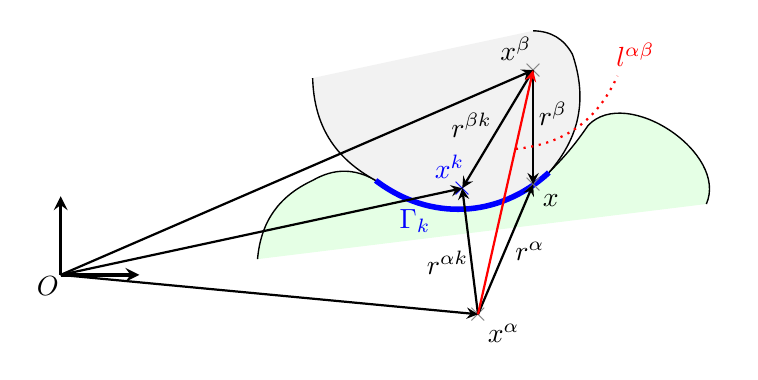
\begin{tikzpicture}
	\coordinate (O) at (-2,-.5);
	\draw[->, >=stealth, very thick] (O) -- ++(1,0);
	\draw[->, >=stealth, very thick] (O) -- ++(0,1);
	\draw (O)++(0.1, 0.1) node[below left]{$O$};
	\coordinate (k_start) at (2, 0.7);
	\coordinate (k_end) at (4.2, 0.8);
	\filldraw[fill=green!10, line width=.05em] (0.5, -0.3) to[bend left] (1.2, 0.7) to[bend left=30] (k_start) to[bend right=40] (k_end) to[bend right=5] ++(0.5, 0.6) to[bend left=80] ++(1.5, -1.);
	\filldraw[fill=gray!10, line width=.05em] (1.2, 2) to[bend right] (k_start) to[bend right=40] (k_end) to[bend right] ++(0.3, 1.5) to[bend right] ++(-.5, 0.3);
	\draw[line width=.2em, color=blue] (k_start) to[bend right=40] (k_end);
	\node[color=gray] (x_alpha) at (3.3, -1) {$\times$};
	\node[color=gray] (x_beta) at (4.0, 2.1) {$\times$};
	\node[color=blue] (x_k) at (3.1, 0.6) {$\times$};
	\node[color=gray] (x) at (4, 0.65) {$\times$};
	\draw[->, >=stealth, thick] (O) -- (x_alpha.center);
	\draw[->, >=stealth, thick] (O) -- (x_beta.center);
	\draw[->, >=stealth, thick] (O) -- (x_k.center);
	\draw[->, >=stealth, thick] (x_beta.center) -- (x_k.center);
	\draw[->, >=stealth, thick] (x_alpha.center) -- (x_k.center);
	\draw[->, >=stealth, thick] (x_beta.center) -- (x.center);
	\draw[->, >=stealth, thick] (x_alpha.center) -- (x.center);
	\draw[->, >=stealth, thick, color=red] (x_alpha.center) -- (x_beta.center);
	\draw (x_alpha) node[below right]{$x^\alpha$};
	\draw (x_beta)++(.1,0) node[above left]{$x^\beta$};
	\draw (x) node[below right]{$x$};
	\draw[color=blue] (x_k)++(0.15,0) node[above left]{$x^k$};
	\draw (3.6,1.4) node[left]{$r^{\beta k}$};
	\draw (3.3,-0.35) node[left]{$r^{\alpha k}$};
	\draw (3.95,1.55) node[right]{$r^{\beta}$};
	\draw (3.65,-0.2) node[right]{$r^{\alpha}$};
	\node[color=red] (l_ab) at (5.3,2.3) {$l^{\alpha\beta}$};
	\draw[color=red, dotted, thick] (3.78,1.1) to[bend right=30] (l_ab.230);
	\draw[color=blue] (2.5,0.45) node[below]{$\Gamma_k$};
\end{tikzpicture}
\caption{\label{annexe:figure_contraintes_moyennes}Illustration géométrique d'un contact $k$ entre une particule $\alpha$ et une particule $\beta$.}
\end{figure}
Pour chaque particule $\alpha$, un point de référence est introduit dont la position, notée $x_j^\alpha$, est arbitraire (cf. figure \ref{annexe:figure_contraintes_moyennes}). En introduisant les notations $x_j^c = x_j^\alpha + r_j^{\alpha c}$ et $x_j = x_j^\alpha + r_j^\alpha$ dans (\ref{annexe:contraintes_final}), la contrainte moyenne devient :
\begin{equation}\label{annexe:contraintes_final_rj}
	\overline{\sigma}_{ij}
	= \cfrac{1}{V} \sum_{\alpha=1}^N \sum_{c=1}^{n_\alpha} \left( f_i^c x_j^\alpha + f_i^c r_j^{\alpha c} \right) + \cfrac{1}{V} \sum_{\alpha=1}^N \sum_{c=1}^{n_\alpha} \int_{\Gamma_c} \left( t_i^{'} x_j^\alpha + t_i^{'} r_j^\alpha \right)\ \mathrm{d} \Gamma_c
\end{equation}
Comme la particule $\alpha$ est à l'équilibre statique, la somme $\sum_{c=1}^{n_\alpha} f_i^c x_j^\alpha = x_j^\alpha \sum_{c=1}^{n_\alpha} f_i^c$ s'annule. D'autre part, l'intégrale $\int_{\Gamma_c} t_i^{'} x_j^\alpha\ \mathrm{d} \Gamma_c = x_j^\alpha \int_{\Gamma_c} t_i^{'}\ \mathrm{d} \Gamma_c$ s'annule par définition de $t_i^{'}$. Cela donne finalement :
\begin{equation}\label{annexe:contraintes_final_rj_2}
	\overline{\sigma}_{ij}
	= \cfrac{1}{V} \sum_{\alpha=1}^N \sum_{c=1}^{n_\alpha} f_i^c r_j^{\alpha c} + \cfrac{1}{V} \sum_{\alpha=1}^N \sum_{c=1}^{n_\alpha} \int_{\Gamma_c} t_i^{'} r_j^\alpha\ \mathrm{d} \Gamma_c
\end{equation}
La double somme ci-dessus peut se ramener à une somme de tous les contacts. Il est alors intéressant de séparer les contacts intérieurs (pour lesquels les deux particules en contact sont à l'intérieur du volume $V$) et les contacts extérieurs (pour lesquels une des deux particules est à l'extérieur). En considérant deux particules $\alpha$ et $\beta$, chaque contact $k$ voit s'exercer sur la surface $\Gamma_k$ :
\begin{itemize}
	\item une force surfacique $t_i^e$ pour les contacts extérieurs, résultant en une force $f_i^{k,e}$ vérifiant $t_i^e = \cfrac{f_i^{k,e}}{\Gamma_k} + t_i^{'e}$ ;
	\item deux forces surfaciques $t_i^{\alpha\beta}$ et $t_i^{\beta\alpha}$ pour les contacts intérieurs, résultant en deux forces $f_i^{\alpha\beta}$ et $f_i^{\beta\alpha}$, et pour lesquelles il est possible d'introduire la même décomposition. Par action-réaction, $f_i^{\alpha\beta} + f_i^{\beta\alpha} = 0$.
\end{itemize}
Pour $n = \sum_{\alpha=1}^N n_\alpha$ contacts dont $n_e$ contacts extérieurs, il est possible d'exprimer la contrainte moyenne sous la forme suivante :
\begin{equation}\label{annexe:sigma_moyen_forces_exterieures}
	\begin{split}
	\overline{\sigma}_{ij}
	= \cfrac{1}{V} \sum_{k=1}^{n-n_e} f_i^{\alpha\beta} r_j^{\alpha k} + f_i^{\beta\alpha} r_j^{\beta k}
	+ \cfrac{1}{V} \sum_{k=1}^{n-n_e} \int_{\Gamma_k} t_i^{'\alpha\beta} r_j^\alpha + t_i^{'\beta\alpha} r_j^\beta\ \mathrm{d} \Gamma_k\qquad\qquad\qquad \\
	+ \cfrac{1}{V} \sum_{\alpha=1}^N \sum_{k=1}^{n_\alpha} r_j^{\alpha k} f_i^{k,e}
	+ \cfrac{1}{V} \sum_{\alpha=1}^N \sum_{k=1}^{n_\alpha} \int_{\Gamma_k} t_i^{'e} r_j^\alpha\ \mathrm{d} \Gamma_k
	\end{split}
\end{equation}
les forces $f_i^{k,e}$ et $t_i^{'e}$ étant nulles partout sauf pour les contacts extérieurs. Les deux premières sommes ne sont effectuées que sur les contacts intérieurs. En appliquant le principe d'action-réaction, (\ref{annexe:sigma_moyen_forces_exterieures}) devient :
\begin{equation}\label{annexe:sigma_moyen_forces_exterieures_2}
	\begin{split}
	\overline{\sigma}_{ij}
	= \cfrac{1}{V} \sum_{k=1}^{n-n_e} f_i^{\alpha\beta} \left( r_j^{\alpha k} - r_j^{\beta k} \right)
	+ \cfrac{1}{V} \sum_{k=1}^{n-n_e} \int_{\Gamma_k} t_i^{'\alpha\beta} \left( r_j^\alpha - r_j^\beta \right)\ \mathrm{d} \Gamma_k\qquad\qquad\qquad \\
	+ \cfrac{1}{V} \sum_{\alpha=1}^N \sum_{k=1}^{n_\alpha} r_j^{\alpha k} f_i^{k,e}
	+ \cfrac{1}{V} \sum_{\alpha=1}^N \sum_{k=1}^{n_\alpha} \int_{\Gamma_k} t_i^{'e} r_j^\alpha\ \mathrm{d} \Gamma_k
	\end{split}
\end{equation}
En définissant :
\begin{itemize}
	\item $l_j^{\alpha\beta} = r_j^\alpha - r_j^\beta = x_j - x_j^\alpha - x_j + x_j^\beta = x_j^\beta - x_j^\alpha$
	\item $l_j^{\alpha\beta} = r_j^{\alpha k} - r_j^{\beta k} = x_j^k - x_j^{\alpha k} - x_j^k + x_j^{\beta k} = x_j^{\beta k} - x_j^{\alpha k}$
\end{itemize}
l'équation (\ref{annexe:sigma_moyen_forces_exterieures_2}) se simplifie :
\begin{equation}\label{annexe:sigma_moyen_forces_exterieures_3}
\begin{split}
\overline{\sigma}_{ij}
= \cfrac{1}{V} \sum_{k=1}^{n-n_e} f_i^{\alpha\beta} l_j^{\alpha\beta}
+ \cfrac{1}{V} \sum_{k=1}^{n-n_e} \int_{\Gamma_k} t_i^{'\alpha\beta} l_j^{\alpha\beta}\ \mathrm{d} \Gamma_k \hspace{5cm} \\
+ \cfrac{1}{V} \sum_{\alpha=1}^N \sum_{k=1}^{n_\alpha} r_j^{\alpha k} f_i^{k,e}
+ \cfrac{1}{V} \sum_{\alpha=1}^N \sum_{k=1}^{n_\alpha} \int_{\Gamma_k} t_i^{'e} r_j^\alpha\ \mathrm{d} \Gamma_k
\end{split}
\end{equation}
Il est à noter alors que :
\begin{equation}\label{annexe:couples_s_annulent}
	\int_{\Gamma_k} t_i^{'\alpha\beta} l_j^{\alpha\beta}\ \mathrm{d} \Gamma_k = l_j^{\alpha\beta} \int_{\Gamma_k} t_i^{'\alpha\beta}\ \mathrm{d} \Gamma_k = 0
\end{equation}
d'où finalement
\begin{equation}\label{annexe:love_weber}
	\overline{\sigma}_{ij}
	= \cfrac{1}{V} \sum_{k=1}^{n-n_e} f_i^{\alpha\beta} l_j^{\alpha\beta}
	+ \cfrac{1}{V} \sum_{\alpha=1}^N \sum_{k=1}^{n_\alpha} r_j^{\alpha k} f_i^{k,e}
	+ \cfrac{1}{V} \sum_{\alpha=1}^N \sum_{k=1}^{n_\alpha} \int_{\Gamma_k} t_i^{'e} r_j^\alpha\ \mathrm{d} \Gamma_k
\end{equation}
ou encore
\begin{equation}\label{annexe:love_weber_2}
	\overline{\sigma}_{ij}
	= \cfrac{1}{V} \sum_{k=1}^{n-n_e} f_i^{\alpha\beta} l_j^{\alpha\beta}
	+ \cfrac{1}{V} \sum_{\alpha=1}^N \sum_{k=1}^{n_\alpha} \int_{\Gamma_k} t_i^{e} r_j^\alpha\ \mathrm{d} \Gamma_k
\end{equation}
\paragraph{}
Pour retrouver alors la célèbre formule de Weber-Love \citep{weber_recherches_1966,love_treatise_1927} (dans sa version sommée sur les contacts), il faut alors supposer que les forces extérieures ($f_i^{k,e}$ et $t_i^{'e}$) sont nulles ou négligeables. Il ne subsiste alors dans l'équation ci-dessus que la première des deux sommes.
\paragraph{}
Dans cette démonstration nous avons introduit la décomposition $t_i = f_i^c/\Gamma_c + t_i^{'}$ afin de mettre en évidence la contribution du moment de contact en présence de surfaces de contact éventuellement importantes. Nous constatons finalement que la contrainte moyenne ne dépend que de la force résultante et non du moment.